\section{Protocols}
\subsection{Hypotheses, margins, and statistical methods}
The first campaign's H1 tests a decreasing $S$ across the four non-legacy doses using the one-sided exact Page test~\cite{page1963}, blocked by triplet. H2 uses two one-sided tests (TOST)~\cite{schuirmann1987,lakens2017} on paired log Lease/Snapshot ratios. It reports exponentiated 90\% paired-$t$ CIs and applies Holm correction~\cite{holm1979} separately to ten write, fourteen read, and four publication lock-wait p99 tests. An adjusted $p<0.05$ establishes equivalence; a CI wholly beyond a margin is classified not equivalent, and other outcomes are inconclusive. H3 reports two-sided 95\% paired-$t$ CIs under Churn without a directional prediction. Descriptive ratios use 95\% CIs. Percentile bootstrap sensitivity~\cite{efron1979} uses 10,000 resamples and fixed seeds; it does not replace the planned tests. Cells are not pooled, and no planned write-zero adjustment was needed.

The margin is fixed before data at $\pm\ln(1/0.90)$, or ratios $[0.90,1/0.90]$, described here as $\pm10\%$ on the multiplicative scale. It is the author's judgment of a difference small relative to the complexity difference between designs, chosen so ten pairs could resolve it. It is not derived from a production requirement. The pre-registration used a pilot standard deviation of paired log ratio near 0.06, giving an expected 90\% CI half-width near 0.035 at ten pairs. Full CIs let readers apply a tighter margin.

The new campaigns preserve this method while defining their own families. The compaction primary hypothesis (H-C) predicts equivalence in all six on cells for each of writes and reads, with separate six-test Holm families; off cells form separate reference families. The table-count trend hypothesis (H-T1) uses four Page tests, one per reader-count and writer-count combination, with Holm across those four. Its equivalence families (H-T2) contain sixteen read and eight applicable write tests. H-T2 predicts equivalence at four tables for each applicable outcome and non-equivalence for reads at 256 tables without a writer. The intervention has five paired units per cell and 95\% CIs without multiplicity correction, as specified before data.

The paced-load primary hypothesis (H-P1) predicts an increasing CoarseLock/Lease write response p99 ratio with delay, using four Page tests and Holm across the load-fraction and reader-mode combinations. H-P2 predicts below-capacity write-throughput equivalence in six cells; H-P3 predicts equivalence at zero delay and a CoarseLock ratio below the margin at the two higher doses under the higher offered fraction, with separate six-test Holm families. H-P4 predicts Lease/Snapshot throughput equivalence in twelve write and six closed-reader tests, with separate Holm families and no open-reader read-throughput test. Median latency and Lease/Snapshot tails have no prediction. Censored components remain in the primary completion-tail test and are disclosed rather than treated as true p99s.

The settled primary hypothesis (H-M1) predicts a rising CoarseLock/Lease write response p50 ratio with delay at $f=0.2$, using two Page tests with Holm across reader modes. H-M2 predicts non-equivalence, with CoarseLock higher, at 200~$\mu$s and 2~ms in both reader modes. H-M3 predicts that CoarseLock's lock-wait and flush-check p50s each lie in $[1,3]$~ms at 2~ms with closed readers, and Lease's below 0.5~ms, with 95\% $t$ CIs wholly inside each band. H-W predicts CoarseLock/Lease write non-equivalence at 700 writes/s. H-R predicts Lease/Snapshot read and write equivalence in the previously inconclusive cell. H-S is a protocol check that the median largest fsync stays below 40~ms in every $f=0.2$ cell and design. The threshold was raised from \HSDraftMs{} to \HSThresholdMs{}~ms after the calibration trials were seen and before any campaign trial; three of \HSDesignCount{} design-level medians (\HSAboveDraftRange{}~ms) exceed \HSDraftMs{}~ms. The sentinel rule R-check compares 22 metrics with their originals using a 90\% Welch interval on the change, with margin $\ln(1/0.90)$ for throughput and $\ln 1.5$ for tails, and classifies each as unchanged, changed, or inconclusive. A changed metric or a contradicted published class commits us to rerunning that campaign. These hypotheses were generated from earlier data and tested on fresh seeds.

The follow-up primary prediction H-F1 takes, per round and design, the OLS slope with intercept of log reads on log free share across the four F1 write rates. Each of Lease and Snapshot must have its arithmetic mean slope's two-sided \FollowCI{}\% $t$ CI wholly inside \FollowSlopeBand{}; both are required, with no multiplicity adjustment. Write rate is the treatment and free share is measured. The band was a judgment fixed before the campaign data: proportional reads give \FollowOne{}, and the earlier post hoc slopes lay inside it.

H-F2 predicts reads rising as write rate falls, separately for Lease and Snapshot: one-sided Page's $L$, \FollowRounds{} rounds as blocks, cells ordered \FollowRateHigh{}, \FollowRateThird{}, \FollowRateSecond{}, \FollowRateLow{} writes/s, predicted ranks \FollowPageRanks{}, $\alpha=\FollowAlpha$, Holm across the \FollowPageFamily{} tests, using \texttt{page\_trend\_test(method='auto')}. H-F3 predicts Lease/Snapshot read equivalence at \FollowRateLow{}, \FollowRateSecond{}, and \FollowRateThird{} writes/s, with paired log-ratio TOST at $\alpha=\FollowAlpha$, margin \FollowMargin{}, exponentiated \FollowCI{}\% paired-$t$ CIs, and one \FollowRatioFamily{}-test Holm family. The \FollowRateHigh{} writes/s comparison has no prediction because it was previously inconclusive twice; it is descriptive.

H-F4 predicts, for CoarseLock in the Mixed histogram cell, arithmetic mean trial shares, as fractions of the trial's reads, of at least \FollowRegionMin{} (20\%) below \FollowFastBound{}~$\mu$s and at or above \FollowBlockedBound{}~$\mu$s, and at most \FollowValleyMax{} (10\%) between those bounds. The result tables report the same shares as percentages, so a valley share of 0.11\% lies far below the 10\% ceiling. Each two-sided \FollowRegionCI{}\% $t$ CI must lie wholly on the predicted side; all three must hold, with no Holm family. Lease and Snapshot's shares are descriptive. The region bounds and share thresholds were judgments fixed before the campaign data; the region bounds drew on first-campaign percentiles already seen. A bucket belongs to the region containing its lower bound, including buckets crossing a boundary. Protocol check H-X predicts no measured flush in any F1 or fsync-off F3 trial. Any flush is reported and the trial retained; H-F1 is then reported both with and without that round, with the inclusive analysis remaining the frozen one.

The five-round design pairs both conditions in CoarseLock and Lease within each cell. P1 predicts CoarseLock's arithmetic mean $q$ in $[1.90,2.10]$ under two acquisitions and $[0.90,1.10]$ under one, in all eight cells. P2 predicts that removing the acquisition lowers CoarseLock's read ratio relative to Lease at delays up to 200~$\mu$s: the 95\% paired-$t$ CI of the ratio of read ratios must lie wholly below one in six cells. These are unadjusted five-pair comparisons, of descriptive strength as specified in the protocol. P3 predicts cycle error within $\pm15\%$ for both conditions, using two waits or one as appropriate, and a CoarseLock write improvement with its 95\% CI above one at 200~$\mu$s and 2~ms.

R-check is the paper name for the settled sentinel rule stored under frozen JSON key \texttt{H\_C} in \path{research/experiments/phase_i7/X_READCOST/analysis_settled/x_settled_results.json}. The frozen \path{research/experiments/phase_i7/X_SETTLED_PREREGISTRATION.md} calls it the sentinel rule H-C; that historical name maps to R-check here. Compaction H-C retains its hypothesis name and is a separate test. R-check's unchanged, changed, and inconclusive categories use the 90\% Welch CI on the new minus original mean paired log ratio; a changed metric or a contradicted published class triggers a rerun, while inconclusive does not rule out change. Class contradiction means a previously equivalent outcome has a new unadjusted interval wholly outside the throughput margin, or a previously not-equivalent outcome has one wholly inside. These trigger checks are not Holm-adjusted and compare combined changes in pause, date, binary, and seeds.

The remaining measurements preserve their original descriptive status. Cells are not pooled. Median and tail trends outside the declared predictions, stall and backlog comparisons, and the earlier fsync and hold-share accounts remain exploratory; tracing outcomes are not covariates fixed before treatment.

\subsection{Campaign cells and auxiliary measurements}
The seven campaigns deliberately extend the lifetime activity covered by the initial measurements. Table~\ref{tab:coverage} counts diagnostics from trial envelopes, including drain. Mixed includes the nine anchor trials and had at most one flush per trial. Publication and Churn exercised reader-set publication, but the first campaign and the intervention ran no compactions because the compaction trigger was disabled. Since Lease and Snapshot differ most when reader sets change, throughput equivalence in a mostly stable set did not establish equivalence under file retirement. The compaction campaign was run to close that gap.

The intervention isolates acquisition count in eight Mixed-shaped cells: two reader counts and four non-legacy doses. It compares the default two-acquisition commit with a one-acquisition commit below the flush threshold in CoarseLock and Lease. Five rounds share a seed across each four-run cell-round unit, giving 160 trials. The default condition is rerun in the same session rather than borrowed from the first campaign. Snapshot is omitted. Section~\ref{sec:intervention} gives the predictions and exact change.

The compaction campaign uses Churn-shaped cells with $r\in\{4,16\}$, $d\in\{0,200,2000\}\,\mu$s, and compaction on or off. On uses a fixed 250~ms timer that merges all active tables into one; calls with at most one table do no work. Twelve cells, three designs, and ten rounds give 360 trials. On and off share seeds within the same reader-count, delay, and round. The implementation has a disclosed asymmetry: CoarseLock and Lease open compaction inputs under the exclusive lock, whereas Snapshot opens them outside all locks. This is not an inherent requirement of leasing.

The table-count campaign removes overlapping-table search as a factor by constructing disjoint ranges. It crosses $N\in\{4,16,64,256\}$, $r\in\{4,16\}$, and zero or one free-running writer. Sixteen cells, three designs, and ten rounds give 480 trials. The fixed 10,240-key space yields 2,560, 640, 160, or 40 keys per initial table. Delay is zero, the memtable threshold is 1~MiB, and no compaction is scheduled. A writer may still flush, so the analysis retains initial and final counts. All designs perform up to $N$ in-memory range comparisons, under the manager lock only in CoarseLock.

Separate lifecycle microbenchmarks in the table-count results measure capture/release at one and sixteen goroutines and uncontended publication from $N$ to $N+1$ tables. They exclude table search, memory-tier lookup, and disk I/O. Lease's test helper mirrors its scratch-copy and lease path; Snapshot uses its production pin/release path. The publication benchmark includes immediate retirement of an unpinned old Snapshot set; Lease models amortized append with spare slice capacity. Scratch is primed before timing. We report the arithmetic mean of three benchmark counts, separately from campaign throughput, without confirmatory tests.

The paced-load campaign tests whether the saturated-writer results persist at a fixed offered rate. It uses sixteen readers, one paced writer, three delay levels, two fractions of earlier Lease write capacity, and closed or open readers, with no compaction. Twelve cells over ten three-design rounds give \PacedTrialCount{} trials. The frozen rates are listed below; Section~\ref{sec:method} defines service time, response time, and censored completion tails.

The settled campaign repeats selected comparisons with a 20~s pause before every trial, after the diagnosis in Section~\ref{sec:settled}. It has nine paced cells: three delays at $f=0.2$ with closed and open readers; 700 writes/s at 200~$\mu$s with closed and open readers, a rate chosen so earlier CoarseLock capacity was \SettledHWFraction{} of the offered rate; and the closed zero-delay $f=0.8$ cell whose read comparison had been inconclusive. Ten three-design rounds give 270 trials, with commit-phase timing, a 1~ms heartbeat goroutine, and per-reader slowest-read tracking enabled. Sentinel cells copy specifications from each earlier campaign without that tracing and add 200 trials, for \SettledTrialCount{} in total, all on fresh seeds.

The follow-up campaign has \FollowCells{} cells and \FollowTrials{} trials, with \FollowRounds{} paired rounds per cell. Its \FollowPacedCells{} paced cells use Lease and Snapshot, closed readers with $r=\FollowReaders$, one writer, and zero delay. The four F1 cells vary intended writes over \FollowRateLow{}, \FollowRateSecond{}, \FollowRateThird{}, and \FollowRateHigh{} writes/s. Their \FollowMemLarge{}~MiB memtable keeps flushes out of the measured windows. F2 changes only that threshold to \FollowMemSmall{}~MiB at \FollowRateHigh{} writes/s. F3 turns fsync off at \FollowRateHigh{} writes/s with the \FollowMemLarge{}~MiB threshold. F4 copies the first campaign's four-reader, zero-delay Mixed cell for CoarseLock, Lease, and Snapshot, adding full read histograms. The paced cells retain commit-phase traces; F4 has no trace, so its hold share is unavailable.

The Paced workload fixes $r=16$ and uses one paced writer, four initial tables, no compaction, and a 10~s measurement window. It crosses $d\in\{0,200,2000\}\,\mu$s, offered write fractions $f\in\{0.2,0.8\}$ of earlier Lease saturated capacity, and closed or open readers. Twelve cells, three designs, and ten rounds give \PacedTrialCount{} trials. The frozen write rates at the three doses are \PacedRatesZero{}, \PacedRatesMedium{}, and \PacedRatesHigh{} writes/s, respectively, with each pair ordered $f=0.2/0.8$; open-reader rates are \PacedOpenRates{} reads/s. The higher write fraction is below CoarseLock's earlier capacity at zero delay and above it at 200 and 2000~$\mu$s. 

The delay probe separates nominal dose from realized lookup time. The earlier single-goroutine probe measured approximately 9, 35, and 215~$\mu$s and 2.25~ms per read; concurrent lock holds are reported separately. The sub-millisecond dose yields while spinning; the 2~ms dose sleeps before a final 0.5~ms spin.

\subsection{Revisions, plans, runners, and seeds}
The first campaign used revision \texttt{c53ee5b}, plan SHA-256 prefix \texttt{68ad96f878c1}, and runner prefix \texttt{22060ffc4885}. The intervention used \texttt{4c2749b}, plan \texttt{2e44fcacb3e7}, and runner \texttt{5dc57e7d85d7}. The compaction campaign used \texttt{c342832}, plan \texttt{5330cbddf01b}, and runner \texttt{3a05470d307b}. The table-count campaign used \texttt{adf754b}, plan \texttt{0bc0042b8b8a}, and runner \texttt{050c3210e9e8}. Protocols are \path{research/experiments/phase_i7/X_PREREGISTRATION.md}, \path{research/experiments/phase_i7/X_INTERVENTION_PREREGISTRATION.md}, \path{research/experiments/phase_i7/X_COMPACTION_PREREGISTRATION.md}, and \path{research/experiments/phase_i7/X_TABLECOUNT_PREREGISTRATION.md}.

The paced-load campaign used revision \texttt{6833d7c}; its design was frozen in \texttt{54572b2}, and the later commit changed only notes. Its plan SHA-256 prefix is \texttt{384aace771c8}, runner prefix \texttt{00f97d04191b}, and protocol \path{research/experiments/phase_i7/X_PACED_PREREGISTRATION.md}. The separate non-campaign append/fsync probe is recorded in \path{research/experiments/phase_i7/X_READCOST/fsync_probe.py} and \path{research/experiments/phase_i7/X_READCOST/fsync_probe.txt}; it was not rerun for this paper update.

The settled campaign's design was frozen at revision \texttt{54b2c67}, with plan SHA-256 prefix \texttt{\SettledPlanPrefix}, runner prefix \texttt{\SettledRunnerPrefix}, and protocol \path{research/experiments/phase_i7/X_SETTLED_PREREGISTRATION.md}. Exploratory evidence, excluded from every campaign analysis, is in \path{research/experiments/phase_i7/X_READCOST/stall_diag/} and \path{research/experiments/phase_i7/X_READCOST/fsync_checks/}, with the narrative in \path{research/experiments/phase_i7/X_READCOST/OVERNIGHT_NOTES.md}. The diagnostic tool's results carry no git revision; the fsync checks used a binary built at \texttt{f71e7e2} with SHA-256 prefix \texttt{d0e7bb68b0a8}.

The follow-up campaign used revision \texttt{\FollowRevision}, plan SHA-256 prefix \texttt{\FollowPlanPrefix}, runner prefix \texttt{\FollowRunnerPrefix}, a \FollowPause{}~s pause, and protocol \path{research/experiments/phase_i7/X_FOLLOWUP_PREREGISTRATION.md}. Results are regenerated from retained raw trials by \path{research/experiments/analysis/x_followup_analyze.py}; \path{research/experiments/analysis/x_followup_paper_outputs.py} reads that JSON and the raw trials to generate the manuscript macros and figures.

Master seeds were 20261030, 20261103, 20261104, 20261105, 20261106, 20261107, and \FollowSeed{}, respectively. Paired seeds are the first eight SHA-256 bytes of decimal master, cell or shared base identifier, and round separated by vertical bars, interpreted as a big-endian signed 64-bit value; compaction on/off shares the base identifier. Plans and ledgers retain execution order, retry and approval bindings, and the excluded smoke runs; the first start stopped after 38 successful trials is disclosed in the protocol.

\section{Full results}
Full cells, uncertainty intervals, and auxiliary results retain their original data captions. Earlier figures keep their original confidence intervals; follow-up descriptive comparisons below use the stated paired intervals. Table macros copy frozen results or the follow-up generator's descriptive calculations.
\begin{table}[t]
\caption{First-campaign cells. The legacy scan has no added delay.}
\label{tab:cells}\centering\scriptsize\setlength{\tabcolsep}{3pt}
\begin{tabular}{lclc}\toprule
Workload & Readers & Injected delay & Cells\\\midrule
Mixed & 4, 16 & 0, 20, 200~$\mu$s, 2~ms, legacy scan & 10\\
Publication & 16 & 0, 200~$\mu$s, 2~ms, legacy scan & 4\\
Churn & 1, 4, 16 & 0 & 3\\\bottomrule
\end{tabular}
\end{table}

\begin{table}[t]
\caption{What the trials exercised in the first six campaigns. Flush counts include drain; compactions count completed work, not no-op timer calls. The follow-up campaign is not in this table; Table~\ref{tab:followuppaced} gives its flushes (none in F1 and F3, one per trial in F2).}
\label{tab:coverage}\centering\small\setlength{\tabcolsep}{3pt}
\begin{tabular}{lrrrr}\toprule
 & Trials & \multicolumn{2}{c}{Flushes/trial} & Total\\
Workload/campaign & & Mean & Max & compactions\\\midrule
\TblCoverageRows
\bottomrule\end{tabular}
\end{table}

\begin{figure*}[t]
\centering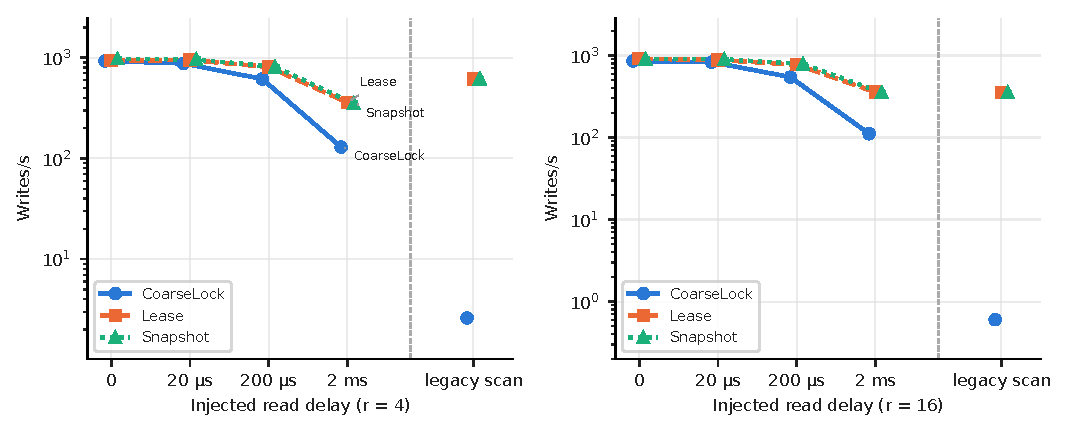
\includegraphics[width=\textwidth]{fig_x1_writes.pdf}
\caption{Mixed workload writes, ten triplets per cell. Points are per-design geometric means; bars are exponentiated 95\% log-$t$ CIs. Most intervals are smaller than the markers. The legacy scan is an isolated category.}
\label{fig:writes}
\end{figure*}

\begin{table*}[t]
\caption{Mixed workload, ten triplets per cell. Rates are geometric means (operations/s); hold is the arithmetic mean of CoarseLock's trial mean read critical sections. Paired ratios have 95\% $t$ CIs.}
\label{tab:x1}\centering\scriptsize\setlength{\tabcolsep}{2pt}
\begin{tabular}{rlr rrr l rrr l}\toprule
 & & Hold & \multicolumn{3}{c}{Writes/s} & $S$ & \multicolumn{3}{c}{Reads/s} & $R_{\mathrm{CL}}/R_{\mathrm{L}}$\\
$r$ & Delay & $\mu$s & CoarseLock & Lease & Snapshot & [95\% CI] & CoarseLock & Lease & Snapshot & [95\% CI]\\\midrule
\TblXOneRows
\bottomrule\end{tabular}
\end{table*}

\begin{figure*}[t]
\centering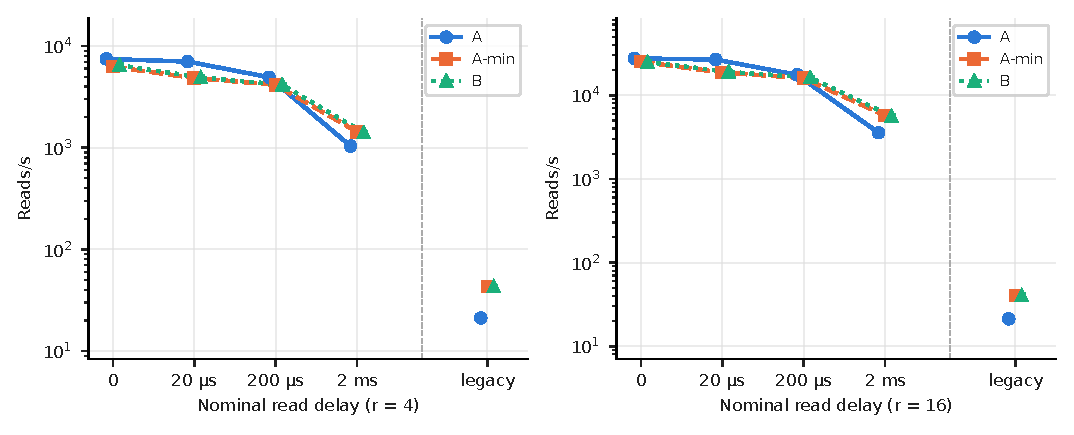
\includegraphics[width=\textwidth]{fig_x1_reads.pdf}
\caption{Mixed workload reads, ten triplets per cell. Points are geometric means; bars are exponentiated 95\% log-$t$ CIs. CoarseLock's low-dose read gain was unpredicted.}
\label{fig:reads}
\end{figure*}

\begin{table*}[t]
\caption{Intervention. $q$ is arithmetic; throughput ratios are paired geometric means, with 95\% paired log-$t$ CIs where shown. Column numbers 2 and 1 denote two-acquisition and one-acquisition commits.}
\label{tab:intervention}\centering\scriptsize\setlength{\tabcolsep}{2pt}
\begin{tabular}{rl rrrr l rr ll}\toprule
 & & \multicolumn{2}{c}{$q_{\mathrm{CL}}$} & \multicolumn{2}{c}{$q_{\mathrm{L}}$} & $W_{\mathrm{CL},1}/W_{\mathrm{CL},2}$ & \multicolumn{2}{c}{$S$} & \multicolumn{2}{c}{$R_{\mathrm{CL}}/R_{\mathrm{L}}$ [95\% CI]}\\
$r$ & Delay & 2 & 1 & 2 & 1 & [95\% CI] & 2 & 1 & 2 & 1\\\midrule
\TblInterventionRows
\bottomrule\end{tabular}
\end{table*}

\begin{figure*}[t]
\centering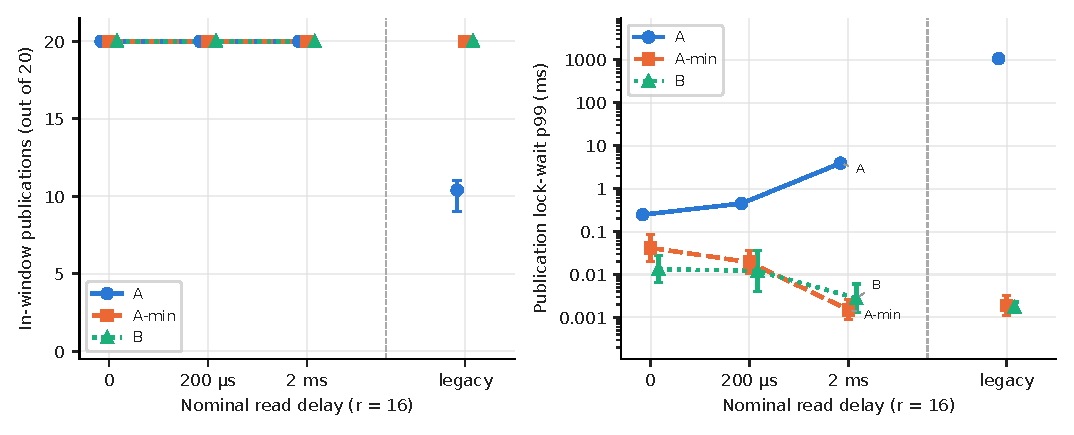
\includegraphics[width=\textwidth]{fig_x2_publication.pdf}
\caption{Publication workload, ten triplets per cell. Left: arithmetic mean in-window count with min--max bars. Right: geometric mean trial publication lock-wait p99 and exponentiated 95\% log-$t$ CIs. Wait counters include drain.}
\label{fig:publication}
\end{figure*}

\begin{table*}[t]
\caption{Publication workload. Rates and trial lock-wait p99 ($\mu$s) are geometric means. Publication counts are median [min, max], out of twenty.}
\label{tab:x2}\centering\scriptsize\setlength{\tabcolsep}{4pt}
\begin{tabular}{l rrr lll rrr}\toprule
 & \multicolumn{3}{c}{Reads/s} & \multicolumn{3}{c}{In-window publications} & \multicolumn{3}{c}{Lock-wait p99 ($\mu$s)}\\
Delay & CoarseLock & Lease & Snapshot & CoarseLock & Lease & Snapshot & CoarseLock & Lease & Snapshot\\\midrule
\TblXTwoRows
\bottomrule\end{tabular}
\end{table*}

\begin{table}[t]
\caption{Publication lock-wait p99: paired Lease/Snapshot ratio, 90\% $t$ CI, and planned classification.}
\label{tab:h2pub}\centering\small\setlength{\tabcolsep}{3pt}
\begin{tabular}{lll}\toprule
Delay & Ratio [90\% CI] & Classification\\\midrule
\TblHTwoPubRows
\bottomrule\end{tabular}
\end{table}

\begin{table*}[t]
\caption{Churn, ten triplets per cell. Rates are geometric means (operations/s). Lease/Snapshot has 95\% paired-$t$ and percentile bootstrap CIs. Flushes are arithmetic means including drain, ordered CoarseLock/Lease/Snapshot.}
\label{tab:x3}\centering\small\setlength{\tabcolsep}{4pt}
\begin{tabular}{rc rrr lll}\toprule
$r$ & Outcome & CoarseLock & Lease & Snapshot & Ratio [95\% $t$ CI] & Bootstrap CI & Flushes\\\midrule
\TblXThreeRows
\bottomrule\end{tabular}
\end{table*}

\begin{table*}[t]
\caption{Compaction-on throughput. Lease/Snapshot ratios have 90\% CIs and Holm-adjusted classifications; $S$ and CoarseLock/Lease read ratios have 95\% CIs. All ratios are paired geometric means.}
\label{tab:compthroughput}\centering\scriptsize\setlength{\tabcolsep}{3pt}
\begin{tabular}{rl ll ll ll}\toprule
 & & \multicolumn{2}{c}{Lease/Snapshot writes} & \multicolumn{2}{c}{Lease/Snapshot reads} & $S$ & $R_{\mathrm{CL}}/R_{\mathrm{L}}$\\
$r$ & Delay & Ratio [90\% CI] & Class & Ratio [90\% CI] & Class & [95\% CI] & [95\% CI]\\\midrule
\TblCompactionThroughputRows
\bottomrule\end{tabular}
\end{table*}

\begin{table*}[t]
\caption{Compaction-on lifecycle measurements. Arithmetic means of trial commit-wait p99 and trial mean retirement lag, including drain.}
\label{tab:complifecycle}\centering\small\setlength{\tabcolsep}{6pt}
\begin{tabular}{rl rrr rrr}\toprule
 & & \multicolumn{3}{c}{Commit-wait p99 ($\mu$s)} & \multicolumn{3}{c}{Mean retirement lag (ms)}\\
$r$ & Delay & CoarseLock & Lease & Snapshot & CoarseLock & Lease & Snapshot\\\midrule
\TblCompactionLifecycleRows
\bottomrule\end{tabular}
\end{table*}

Retirement ran in all on cells in the exploratory lifecycle measurements. Mean retirement lags spanned \CompLagCL{}~ms for CoarseLock, \CompLagL{}~ms for Lease, and \CompLagS{}~ms for Snapshot. Cell mean retired-table high-water marks were \CompHighWater{} across the designs (Table~\ref{tab:complifecycle}). At low doses, counts were roughly timer-limited, with cell means of \CompCountLow{} compactions per trial. At 2~ms they were flush-limited: CoarseLock completed mean counts of \CompCountHighCL{} versus \CompCountHighOther{} in the alternatives because it produced fewer flushes. These observations do not establish compaction starvation.

\begin{table*}[t]
\caption{Table-count campaign, ten triplets per cell. Throughput ratios are Lease/Snapshot with 90\% paired log-$t$ CIs and planned Holm-adjusted classes. CS is arithmetic mean read critical section ($\mu$s). A dash means no writer and no applicable write test.}
\label{tab:tablecount}\centering\scriptsize\setlength{\tabcolsep}{4pt}
\begin{tabular}{rrr ll ll rrr}\toprule
 & & & \multicolumn{2}{c}{Reads} & \multicolumn{2}{c}{Writes} & \multicolumn{3}{c}{Mean read CS ($\mu$s)}\\
$N$ & $r$ & Writers & Ratio [90\% CI] & Class & Ratio [90\% CI] & Class & CoarseLock & Lease & Snapshot\\\midrule
\TblTablecountRows
\bottomrule\end{tabular}
\end{table*}

\begin{table*}[t]
\caption{Separate lifecycle microbenchmarks: arithmetic mean of three counts, ns/operation. Read-cycle benchmarks allocate no memory. Publication allocation counts are per operation.}
\label{tab:microbench}\centering\small\setlength{\tabcolsep}{6pt}
\begin{tabular}{r rrrr rrrr}\toprule
 & \multicolumn{2}{c}{Read cycle, 1 goroutine} & \multicolumn{2}{c}{Read cycle, 16 goroutines} & \multicolumn{2}{c}{Publication} & \multicolumn{2}{c}{Publication allocations}\\
$N$ & Lease & Snapshot & Lease & Snapshot & Lease & Snapshot & Lease & Snapshot\\\midrule
\TblMicrobenchRows
\bottomrule\end{tabular}
\end{table*}

The exploratory per-table critical-section increase was roughly \TableSlopeFour{}~ns at four readers and \TableSlopeSixteen{}~ns at sixteen, compared with about \BenchSlope{}~ns per table in the single-goroutine microbenchmark. Cold cache lines on real table objects spread through the heap are a possible explanation, not a tested one. The microbenchmark uses synthetic table objects and isolates lifecycle operations; it is not an end-to-end read measurement.

\begin{table*}[t]
\caption{Paced workload, ten triplets per cell. Achieved fractions and write response p50 are arithmetic means of trial summaries. Saturated counts are CoarseLock trials below 0.95 completed/offered. Throughput is the paired geometric CoarseLock/Lease ratio with its frozen 90\% CI and Holm-adjusted H-P2 or H-P3 class. Rounded 1.000 intervals are not exact equality.}
\label{tab:paced}\centering\scriptsize\setlength{\tabcolsep}{3pt}
\begin{tabular}{lrlr rrr r ll rr}\toprule
 & & & Offered & \multicolumn{3}{c}{Achieved write fraction} & Saturated & \multicolumn{2}{c}{CoarseLock/Lease writes} & \multicolumn{2}{c}{Response p50 (ms)}\\
Delay & $f$ & Readers & writes/s & CoarseLock & Lease & Snapshot & CoarseLock & Ratio [90\% CI] & Class & CoarseLock & Lease\\\midrule
\TblPacedRows
\bottomrule\end{tabular}
\end{table*}

\begin{table*}[t]
\caption{Paced descriptive ratios, with frozen 95\% paired log-$t$ CIs. All columns except the last compare CoarseLock/Lease. The read column is throughput for closed readers and response p99 for open readers. The last column compares Lease/Snapshot write response completion-p99, with no prediction; unissued ticks have no observed latency, and censored ratios do not bound true ratios. No median or tail trend test is added.}
\label{tab:paced-descriptive}\centering\scriptsize\setlength{\tabcolsep}{4pt}
\begin{tabular}{lrl llll}\toprule
 & & & \multicolumn{2}{c}{CoarseLock/Lease writes} & CoarseLock/Lease & Lease/Snapshot\\
Delay & $f$ & Readers & Response p50 & Service p50 & Read metric & Response p99\\\midrule
\TblPacedDescriptiveRows
\bottomrule\end{tabular}
\end{table*}

The higher offered fraction was not a comfortable operating point for any design in the exploratory descriptive comparison. For Lease and Snapshot, cell medians of trial write response p99 ranged from \PacedLSTailMedians{}~ms, while cell medians of trial p50 were \PacedLSResponseMedians{}~ms. Even trials above the 0.95 completion flag left up to \PacedUnissuedAboveFlag{} ticks unissued, so the flag understates censoring. The descriptive Lease/Snapshot completion-p99 ratios and wide 95\% CIs are reported in Table~\ref{tab:paced-descriptive}; no prediction or equivalence conclusion applies to them. Their write service p50 ratios stayed at \PacedLSServiceRange{}. Similar service medians do not establish similar response tails.

\begin{table}[t]
\caption{Fsyncs of 25~ms or longer, by write rate. Settled trials are all three designs. Bare runs are exploratory, with no engine. ``No first'' excludes each run's first fsync. The last row's bare runs were at 700 writes/s.}
\label{tab:bursts}\centering\scriptsize\setlength{\tabcolsep}{3pt}
\begin{tabular}{r rr rrr}\toprule
 & \multicolumn{2}{c}{Settled} & \multicolumn{3}{c}{Bare}\\
Writes/s & Trials & Fsyncs (\%) & Runs & No first & Fsyncs (\%)\\\midrule
\TblBurstRows
\bottomrule\end{tabular}
\end{table}

\begin{table*}[t]
\caption{Exploratory fsync on/off check at zero delay, 732 writes/s, closed readers, ten rounds. Ratios are paired geometric Lease/Snapshot means with 90\% CIs. Classes use the declared margin with no multiplicity correction. Rounded 1.000 intervals are not exact equality.}
\label{tab:fsync}\centering\scriptsize\setlength{\tabcolsep}{3pt}
\begin{tabular}{l ll r r ll ll}\toprule
 & \multicolumn{2}{c}{Reads/s} & Trials with fsync & Hold & \multicolumn{2}{c}{Lease/Snapshot reads} & \multicolumn{2}{c}{Lease/Snapshot writes}\\
Fsync & Lease & Snapshot & $\geq25$~ms & (\%) & Ratio [90\% CI] & Class & Ratio [90\% CI] & Class\\\midrule
\TblFsyncRows
\bottomrule\end{tabular}
\end{table*}

\begin{table*}[t]
\caption{Follow-up paced cells, \FollowRounds{} paired rounds each. Reads and achieved writes are arithmetic mean operations/s; hold share and measured flushes are arithmetic means including drain. The Lease/Snapshot read ratio repeats on each design's row and has a descriptive \FollowCI{}\% paired log-$t$ CI.}
\label{tab:followuppaced}\centering\scriptsize\setlength{\tabcolsep}{3pt}
\begin{tabular}{rl l rrrr l}\toprule
Offered writes/s & Fsync, memtable & Design & Reads/s & Writes/s & Hold share & Flushes & Lease/Snapshot [\FollowCI{}\% CI]\\\midrule
\FollowPacedRows
\bottomrule\end{tabular}
\end{table*}

At \FollowRateHigh{} writes/s, the \FollowMemSmall{}~MiB against \FollowMemLarge{}~MiB read ratios were \FollowSmallMemRatioL{} and \FollowSmallMemRatioS{} for Lease and Snapshot (\FollowCI{}\% paired-$t$ CIs), with one flush per trial against none and similar hold share. This comparison is descriptive. Cell mean reads divided by the product of each design's fsync-off median reads and cell mean free share were \FollowCapacityLowL{}/\FollowCapacityLowS{} at \FollowRateLow{} writes/s and \FollowCapacityHighL{}/\FollowCapacityHighS{} at \FollowRateHigh{} (Lease/Snapshot). The paired log-ratio SDs at the four F1 rates were \FollowSDLow{}, \FollowSDSecond{}, \FollowSDThird{}, and \FollowSDHigh{}, and \FollowSDOff{} with fsync off. H-X held: no F1 or F3 trial flushed.

The fixed-rate fsync comparison pairs F3 and F1 at \FollowRateHigh{} writes/s within each round and design. It takes $\ln(R_{\mathrm{F3}}/R_{\mathrm{F1}})$ and $\ln(\mathrm{free}_{\mathrm{F3}}/\mathrm{free}_{\mathrm{F1}})$ and their difference, then exponentiates the mean difference and its two-sided \FollowCI{}\% paired-$t$ CI. Per-round logs and differences are retained in comments in the generated \path{paper/generated/followup.tex}. This exploratory comparison does not change the frozen H-F1 test. The fsync-off read comparison is descriptive, with its \FollowCI{}\% interval inside the margin; it is outside the H-F3 Holm family.

\begin{table}[t]
\caption{Follow-up F1 and F3 cells: arithmetic means of per-trial memtable share and reads/s per unit free share, for Lease and Snapshot. Memtable share divides the whole-trial memory-read counter by completed window-issued reads, including drain.}
\label{tab:memshare}\centering\scriptsize\setlength{\tabcolsep}{3pt}
\begin{tabular}{l rr rr}\toprule
 & \multicolumn{2}{c}{Memtable share} & \multicolumn{2}{c}{$R/\mathrm{free}$ (reads/s)}\\
Offered writes/s & Lease & Snapshot & Lease & Snapshot\\\midrule
\TblMemShareRows
\bottomrule\end{tabular}
\end{table}

A post hoc, untested fit of $1/(R/\mathrm{free})$ on memtable share has \MemFitParameterCount{} parameters on \MemFitCellCount{} F1 cell means per design, Pearson $r=\MemFitPearsonL{}$ for Lease and $r=\MemFitPearsonS{}$ for Snapshot, and fsync-off capacity ratios of \MemFitOffRatioL{} and \MemFitOffRatioS{} (mean $R/\mathrm{free}$ divided by the reciprocal line prediction at its own share); the share is approximate because the two counters do not cover exactly the same interval.

\begin{table}[t]
\caption{Follow-up F1 cells: hold per commit (mean hold share divided by mean achieved writes per second, ms) and the share of the exclusive hold spent in WAL sync (mean of per-trial shares, \%), for Lease and Snapshot. The hold is validation, WAL write, WAL sync, and apply.}
\label{tab:holdpercommit}\centering\scriptsize\setlength{\tabcolsep}{4pt}
\begin{tabular}{r rr rr}\toprule
 & \multicolumn{2}{c}{Hold per commit (ms)} & \multicolumn{2}{c}{WAL sync share (\%)}\\
Offered writes/s & Lease & Snapshot & Lease & Snapshot\\\midrule
\TblHoldPerCommitRows
\bottomrule\end{tabular}
\end{table}

\begin{table}[t]
\caption{Follow-up Mixed read-latency region shares, arithmetic mean trial percentages [\FollowRegionCI{}\% $t$ CI], using bucket lower bounds. H-F4 applies to CoarseLock only and held: its thresholds are at least 20\% in the fast and blocked regions and at most 10\% in the valley.}
\label{tab:followupregions}\centering\scriptsize\setlength{\tabcolsep}{2pt}
\begin{tabular}{llll}\toprule
Design & Fast & Valley & Blocked\\\midrule
\FollowRegionRows
\bottomrule\end{tabular}
\end{table}

The arithmetic means of per-trial slow-group medians were \FollowSlowMedianA{}, \FollowSlowMedianL{}, and \FollowSlowMedianS{}~$\mu$s for CoarseLock, Lease, and Snapshot, respectively, assigning each sample to its bucket's lower bound. These are conditional on the slow group and are descriptive; the cell has no commit-phase trace.
\begin{figure}[t]
\centering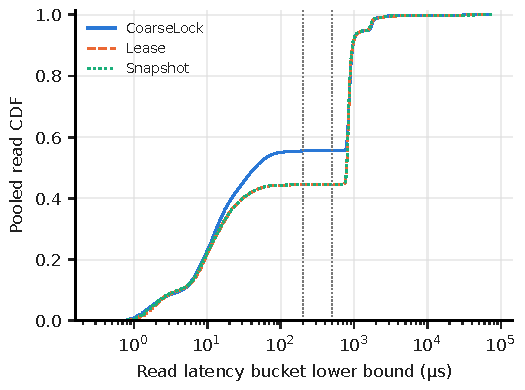
\includegraphics[width=\columnwidth]{fig_read_cdf.pdf}
\caption{Follow-up Mixed read-latency CDFs, all three designs, \FollowRounds{} rounds pooled by summing histogram bucket counts, with mass at each bucket's lower bound. The log latency axis is in $\mu$s; dotted verticals mark \FollowFastBound{} and \FollowBlockedBound{}~$\mu$s. H-F4's regions use these lower bounds; within-bucket timings are unavailable.}
\label{fig:readcdf}
\end{figure}

\begin{figure}[t]
\centering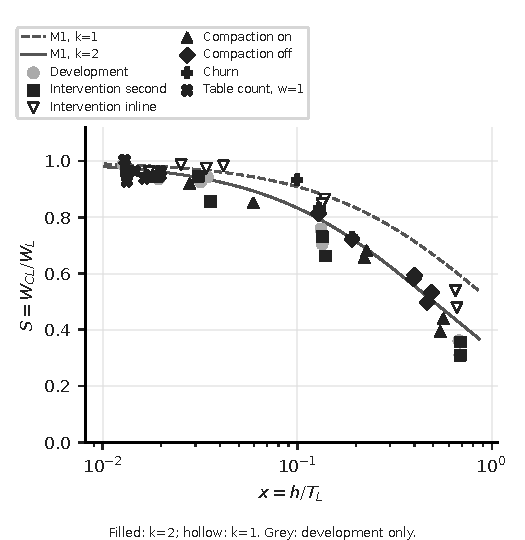
\includegraphics[width=\columnwidth]{fig_penalty_collapse.pdf}
\caption{Exploratory collapse check: write ratio against CoarseLock's mean read hold over Lease's commit cycle, with $S=1/(1+kx)$ drawn for $k=1$ and $k=2$. Filled markers have $k=2$, hollow $k=1$; grey cells were seen before the criteria were written and do not count. Neither model met the criteria.}
\label{fig:collapse}
\end{figure}

\begin{figure}[t]
\centering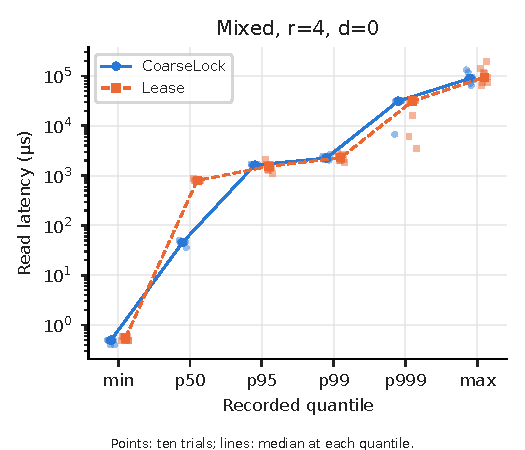
\includegraphics[width=\columnwidth]{fig_read_quantiles.pdf}
\caption{Stored read-latency percentiles, Mixed, $r=4$, zero delay, ten trials per design, with a median line. Trials stored percentiles and no histograms, so this cannot establish modes; Fig.~\ref{fig:readcdf} shows the full histograms from the follow-up campaign.}
\label{fig:readquantiles}
\end{figure}

\begin{figure*}[t]
\centering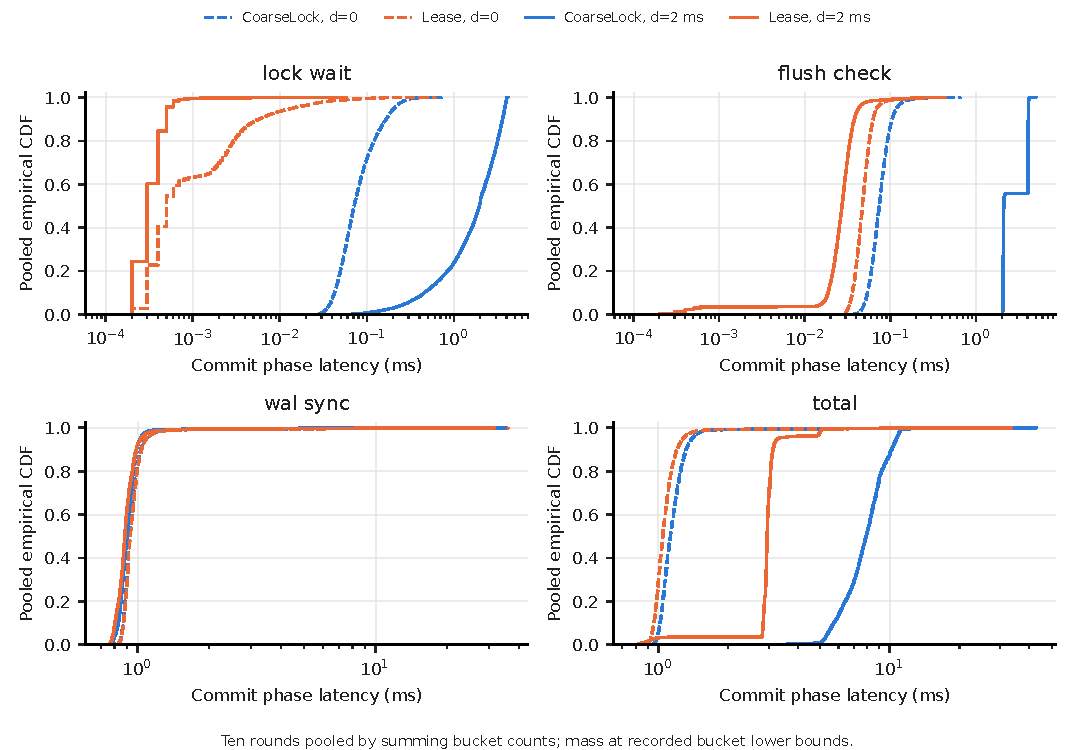
\includegraphics[width=\textwidth]{fig_commit_cdf.pdf}
\caption{Commit-phase empirical CDFs from the settled campaign, closed readers, ten rounds pooled by summing bucket counts, with mass at each bucket's lower bound. Exploratory.}
\label{fig:commitcdf}
\end{figure*}

\begin{figure}[t]
\centering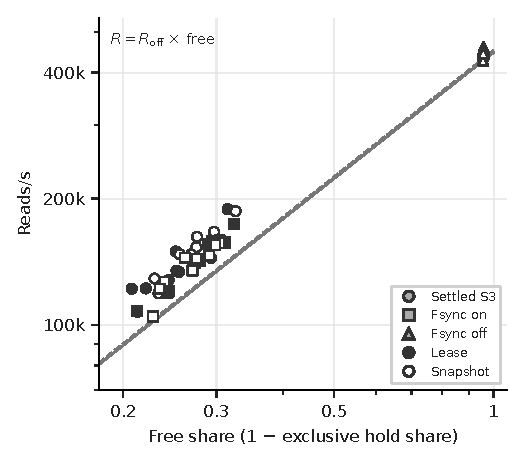
\includegraphics[width=\columnwidth]{fig_hold_reads.pdf}
\caption{Reads against the share of the window outside the writer's exclusive hold, zero delay, 732 writes/s, closed readers, log axes. Post hoc, exploratory. The line is fsync-off median capacity scaled by free share.}
\label{fig:hold}
\end{figure}

\section{Project history and execution notes}
\subsection{Earlier measurements}
A defective reader motivated the present study but supplies no pooled evidence for it. That reader scanned from the target block toward the data end, used about four unbuffered syscalls per record, and did not stop after passing the target key. A 960-trial WSL2 campaign comparing CoarseLock and Snapshot and a Windows campaign stopped by its stopping rule at 60 of 330 planned trials, with 18 complete triplets, used this path. They reported Snapshot completing 3.3--18.5 times CoarseLock's writes and churn throughput ratios of 0.63--0.74 at $r\leq4$. We retain the defective path only as the legacy scan operating point. The earlier campaigns motivated the controlled delay, were not pooled with these data, and carry no inference into this paper. This study supersedes their claims, including the withdrawn $\pm5\%$ equivalence claim and any earlier claim about Lease under churn.

\subsection{Smoke trials and aborted starts}
The earlier campaigns' smoke trials preceded their freezes and were excluded. The first campaign had 21 smoke trials before analysis rules were fixed; the intervention had eight after predictions were written; compaction had fifteen; table count had six; paced load had six after predictions were written. The settled campaign had six mechanical smoke trials before its freeze, from a dirty tree with an earlier runner build, with outcomes unread, and 36 non-campaign calibration trials whose outcomes were seen. After seeing that calibration and before any campaign trial, we raised the H-S threshold from 25 to 40~ms. The table-count single-round smoke ratio near 0.66 at 256 tables and sixteen readers pointed in the predicted direction, although predictions were written first. No design value, margin, or prediction changed because of these runs. An operator also stopped the first start at 38 of 519 trials for power-supply reasons unrelated to results. It was discarded without analysis; only status lines were seen. Fixtures were constructed without fsync.

The follow-up had \FollowSmoke{} mechanical smoke trials after its freeze, excluded from analysis, with only status, trace and histogram presence, cleanup, and ledger checked. An aborted start stopped at the operator's request after a leftover process had to be closed during the run: \FollowAbortedFinished{} trials finished and the \FollowAbortedKilled{}th was killed in flight. The records were set aside unread and excluded; only status lines were seen. The campaign restarted from trial \FollowOne{} with the same plan, seeds, and runner in a fresh folder. All \FollowSuccesses{} of \FollowTrials{} retained trials succeeded on the first attempt, with no retries or dropped traces and gaps of \FollowGapMin{} to \FollowGapMax{}~s. The host was on AC power at the start and end, and the machine was left alone during the restarted run.

Four later protocols were frozen and not run for this paper: X-locks, X-inputopen, X-realism, and X-memtable. The repository holds no campaign folder or trial for X-locks, X-inputopen, or X-realism. X-memtable had four mechanical smoke trials, excluded from analysis, and an aborted start stopped at the operator's request after one finished trial; that trial was kept unread and excluded, and the campaign has not been run.

\subsection{Power record and settled execution deviations}
\path{platform.json} records the Balanced base plan. The overnight campaigns ran on AC power with other user applications closed by the operator; the Best performance overlay on the Balanced base plan was read back from the registry after both had finished, not during them. This does not independently verify the overlay throughout execution. Defender and other host activity remain possible sources of variation. The first five campaigns ran back to back, so each trial could inherit host effects from the one before. The settled sentinels bound this only in the rechecked cells, and they confound the pause with date, binary, and seeds. Bursts near 31~ms were not controlled in any campaign. During the settled campaign a helper process held a power request to prevent idle standby and spawned about 50 short \texttt{tasklist} processes; one read-only status check overlapped one trial, which is the largest of its group and is retained under the no-exclusion rule, though no prediction depends on its tail; the desktop application was also running, and the operator was away, so it cannot be confirmed that the machine stayed untouched.

The settled pause and H-S threshold were selected after non-campaign calibration. Its 36 seen trials were excluded from campaign inference, and its six mechanical smoke trials used a dirty tree and an earlier runner build with outcomes unread. No campaign trial preceded the change from the draft 25~ms H-S threshold to 40~ms. The overlapping status check, helper activity, and desktop application described above remain execution deviations, with the affected trial retained under the no-exclusion rule.

\subsection{Race-detector context}
The race detector reported no data races in the engine and campaign harness tests under Linux on WSL2, rerun after commit-phase tracing was added; one older overload test fails under the detector for a timing reason because the slowdown disturbs the overload it expects. The older timing-sensitive failure is the E4 overload test. This was not a Windows race-detector run.

The trial runner \texttt{i7trial}, which \texttt{xcampaign} takes through its \texttt{-runner} flag, builds for linux/amd64 from the Windows checkout (\texttt{GOOS=linux GOARCH=amd64 go build} completed without error, as did the \texttt{xcampaign} build). We ran no trial on Linux, and no Linux result appears here.
